\documentclass[journal]{IEEEtran}

\usepackage[T1]{fontenc}
\usepackage{graphicx}
\usepackage{amsmath,amssymb}
\usepackage{booktabs}
\usepackage{array}
\newcolumntype{L}[1]{>{\raggedright\arraybackslash}p{#1}}
\usepackage{siunitx}
\usepackage{xcolor}
\usepackage{tikz}
\usetikzlibrary{arrows.meta,positioning,shapes.geometric,calc,fit,backgrounds}
\usepackage{url}
\usepackage[hidelinks]{hyperref}
\usepackage[capitalise,nameinlink]{cleveref}

\sisetup{detect-all, range-phrase=--, range-units=single}
\graphicspath{{figures/}{../media/}}

% colours used in diagrams (same blue/orange/aqua as the charts)
\definecolor{cblue}{HTML}{2A78D6}
\definecolor{corange}{HTML}{EB6834}
\definecolor{caqua}{HTML}{1BAF7A}
\definecolor{cgray}{HTML}{52514E}
\definecolor{cfill}{HTML}{EEF4FC}

\tikzset{
  box/.style={draw=cgray, rounded corners=2pt, fill=cfill, align=center,
              font=\scriptsize, inner sep=3pt, minimum height=0.55cm},
  decision/.style={draw=cgray, diamond, aspect=2.2, fill=white, align=center,
              font=\scriptsize, inner sep=1pt},
  stop/.style={draw=corange, rounded corners=2pt, fill=corange!12, align=center,
              font=\scriptsize, inner sep=3pt},
  term/.style={draw=cgray, rounded corners=7pt, fill=white, align=center,
              font=\scriptsize, inner sep=3pt},
  arr/.style={-{Stealth[length=4pt]}, cgray, line width=0.5pt},
  lbl/.style={font=\tiny, text=cgray, align=center},
}

\begin{document}

\title{Autonomous Mobile Pick-and-Place with a TurtleBot3 and an OpenMANIPULATOR-X in ROS~2 Simulation}

\author{Muhammad~Ali~Sadiq%
\thanks{M.Eng.\ Mechatronics \& Cyber-Physical Systems, Deggendorf Institute of Technology (TH Deggendorf), Germany. Case study report, November 2026.}%
\thanks{Source code, data, scripts and videos: \url{https://github.com/turtleshelp/mobile-robot-with-arm}.}}

\markboth{Case Study Report, M.Eng.\ Mechatronics \& Cyber-Physical Systems, TH Deggendorf, November 2026}%
{Sadiq: Autonomous Mobile Pick-and-Place in ROS~2 Simulation}

\maketitle

\begin{abstract}
This report presents a simulated mobile manipulator that finds a cube, picks it up, carries it across a room and places it on a second pedestal without human input. The robot combines a TurtleBot3 Waffle Pi base with a four-joint OpenMANIPULATOR-X arm and runs on ROS~2 Humble, Gazebo Classic~11, Nav2 and MoveIt~2. Because Nav2 alone stops only within about \SI{10}{cm} of a goal, parking is split into two stages: Nav2 drives to a staging pose, and a LiDAR docking step fits a line to the pedestal face and aligns the robot to it. An RGB-D camera locates the cube by colour and depth, and the arm grasps it with analytic inverse kinematics along straight-line paths. Over 17 logged runs, docking reduced the sideways parking error at the drop pedestal from a mean of \SI{7.2}{cm} to \SI{1.2}{cm}, and the camera located randomly placed cubes within \SIrange{1.0}{3.2}{mm}. Thirteen runs ended with the cube on the drop pedestal according to the simulator. Three were stopped safely by the robot's own checks, and one failed undetected when the physics engine became unstable while the gripper opened. The results show that a small, mostly deterministic pipeline can do the task reliably in simulation. They also show where its evidence ends: grasping relies on a simulation-only attachment plugin, and the sample is small.
\end{abstract}

\begin{IEEEkeywords}
Mobile manipulation, ROS~2, Nav2, MoveIt~2, Gazebo, LiDAR docking, RGB-D perception, inverse kinematics.
\end{IEEEkeywords}

% =====================================================================
\section{Introduction}

\IEEEPARstart{M}{obile} manipulators combine a driving base with a robot arm, so that one machine can both move through a building and handle objects. They are studied for intralogistics, machine tending and service robotics, where parts must be fetched from one place and delivered to another~\cite{hvilshoj2012aimm}. Even in its simplest form the task links several hard problems: the robot has to know where it is, drive there, park precisely enough for a short arm to reach, find the object, grasp it and set it down again.

This case study builds such a system end to end in simulation, using standard open-source components where they fit and small purpose-built parts where they do not. The concrete task is: \emph{starting from a known pose, fetch a \SI{4}{cm} red cube from one pedestal and place it on another pedestal on the far side of a 6\,m $\times$ 5\,m room}.

\subsection{Objectives and scope}
\begin{enumerate}
  \item A complete, autonomous pick-and-place mission started by one launch command and one mission node.
  \item Parking accurate enough for the small OpenMANIPULATOR-X, which grasps about \SI{20}{cm} in front of the base within a window only a few centimetres deep.
  \item Locating the cube with an on-board camera rather than assuming its position.
  \item Safety checks that stop the mission before the arm moves if the situation is not as expected.
  \item An honest evaluation with ground truth from the simulator, and a repository that others can rebuild from scratch.
\end{enumerate}
The work is simulation only. A real robot, multiple or unknown objects, and dynamic obstacles are out of scope.

\subsection{Contributions}
The main contributions are a two-stage parking method (Nav2 plus LiDAR line-fit docking), a camera-based cube localization pipeline that works from the staging pose, a deterministic grasping scheme with analytic inverse kinematics and straight-line motions, a set of run-time safety checks, and an evaluation over 17 logged runs that includes the failures. All code, data and scripts are public~\cite{repo}.

% =====================================================================
\section{Background}

\subsection{ROS~2 and middleware}
ROS~2~\cite{macenski2022ros2} structures a robot's software as nodes that communicate over topics, services and actions, on top of the Data Distribution Service (DDS). The DDS implementation can be chosen at run time. This project uses Eclipse Cyclone DDS~\cite{cyclonedds}, for the reason given in \cref{sec:problems}.

\subsection{Localization and navigation}
The map is built offline with SLAM Toolbox~\cite{macenski2021slam}. At run time the robot is localized with AMCL, an adaptive Monte Carlo (particle filter) localization method~\cite{fox1999mcl,thrun2005probabilistic}, and driven with Nav2~\cite{macenski2020marathon}. Nav2 plans a global path on a costmap and follows it with a local controller. Here the controller is Regulated Pure Pursuit~\cite{macenski2023rpp}, wrapped by a rotation shim that first turns the robot towards the path.

\subsection{Manipulation and simulation}
MoveIt~2~\cite{coleman2014moveit} provides motion planning with sampling-based planners such as RRT-Connect~\cite{kuffner2000rrtconnect}. The simulation runs in Gazebo Classic~11~\cite{koenig2004gazebo} with the ODE physics engine~\cite{ode}, and the joints are driven through \texttt{ros2\_control}, the ROS~2 successor of \texttt{ros\_control}~\cite{chitta2017roscontrol}. Images are processed with OpenCV~\cite{bradski2000opencv}.

\subsection{Grasping in Gazebo Classic}
Physics engines are known to struggle with stable grasps of small objects: contact forces between light fingers and the object can build up and push the object away. A common workaround in Gazebo Classic is a ``grasp fix'' plugin that attaches the object to the gripper with a fixed joint once a grasp is detected~\cite{buehler_grasp}. This project uses its own minimal version of that idea (\cref{sec:grasp}).

% =====================================================================
\section{System Design}

\subsection{Robot and environment}
\begin{figure}[t]
  \centering
  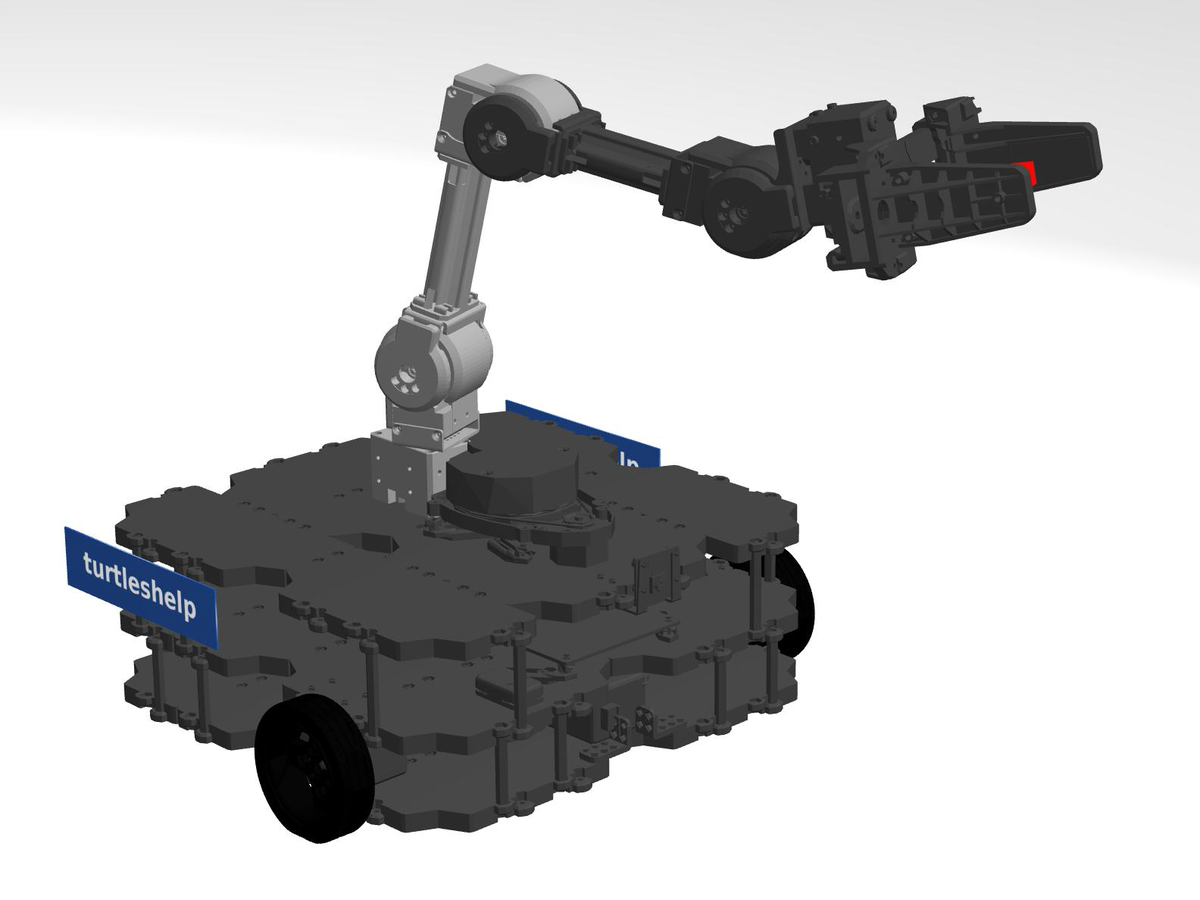
\includegraphics[width=0.85\columnwidth]{robot.png}
  \caption{The simulated robot: TurtleBot3 Waffle Pi base with a 2D LiDAR and an RGB-D camera, and a 4-DOF OpenMANIPULATOR-X arm with a two-finger gripper (rendered in Gazebo).}
  \label{fig:robot}
\end{figure}

The robot (\cref{fig:robot}) is the ROBOTIS TurtleBot3 Waffle Pi differential-drive base~\cite{robotis_tb3} with the OpenMANIPULATOR-X arm~\cite{robotis_omx}, taken from the ROBOTIS \texttt{turtlebot3\_manipulation} description at a fixed commit~\cite{robotis_tb3manip}. The base carries a 360° 2D LiDAR. An RGB-D camera was added at the position of the Waffle Pi's camera (640\,$\times$\,480\,px, \SI{62}{\degree} horizontal field of view, \SI{10}{Hz}, Gaussian depth noise with $\sigma = \SI{5}{mm}$).

The world is a walled 6\,m $\times$ 5\,m arena with three box obstacles and two pedestals of 0.25\,$\times$\,0.25\,$\times$\,0.18\,m: the pickup pedestal at $(2.30, -0.30)$ and the drop pedestal at $(-2.30, 0)$. The \SI{4}{cm}, \SI{30}{g} cube starts on the pickup pedestal about \SI{1}{cm} behind its front face. The gripper opens to about \SI{8.8}{cm}.

\subsection{Software architecture}
\Cref{fig:arch} shows the main nodes. One launch file starts Gazebo with the robot and its controllers, the map server and AMCL, Nav2, MoveIt~2 and the cube detector. The mission node then runs the task as a fixed sequence. It talks to Nav2 through the \texttt{navigate\_to\_pose} action, to the arm controller through a \texttt{FollowJointTrajectory} action, and to the gripper through an effort command topic. It reads the LiDAR scan, odometry and the detector's cube position directly.

\begin{figure*}[t]
\centering
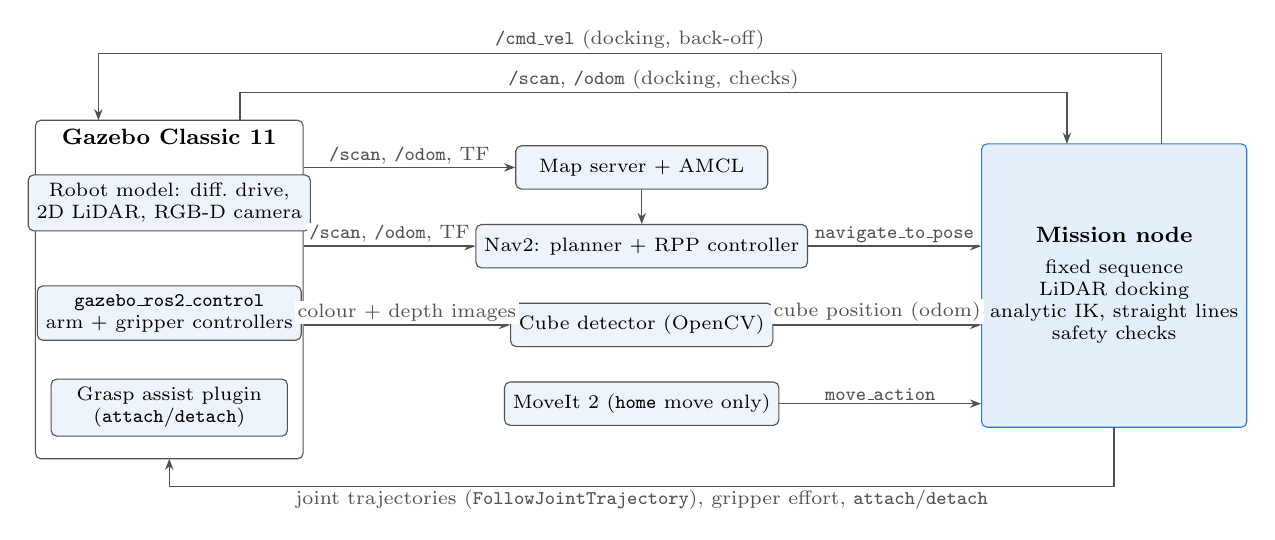
\begin{tikzpicture}[font=\scriptsize,
  al/.style={font=\scriptsize, text=cgray, fill=white, inner sep=1pt}]
  % Gazebo (left)
  \node[box, fill=white, minimum width=3.4cm, minimum height=4.3cm] (gz) at (0,2.05) {};
  \node[font=\footnotesize\bfseries, anchor=north] at (gz.north) {Gazebo Classic 11};
  \node[box, minimum width=3.0cm] (rob) at (0,3.15) {Robot model: diff.\ drive,\\ 2D LiDAR, RGB-D camera};
  \node[box, minimum width=3.0cm] (rc)  at (0,1.75) {\texttt{gazebo\_ros2\_control}\\ arm + gripper controllers};
  \node[box, minimum width=3.0cm] (ga)  at (0,0.55) {Grasp assist plugin\\ (\texttt{attach}/\texttt{detach})};
  % ROS 2 nodes (middle)
  \node[box, minimum width=3.2cm] (amcl) at (6.0,3.6) {Map server + AMCL};
  \node[box, minimum width=3.2cm] (nav)  at (6.0,2.6) {Nav2: planner + RPP controller};
  \node[box, minimum width=3.2cm] (det)  at (6.0,1.6) {Cube detector (OpenCV)};
  \node[box, minimum width=3.2cm] (mov)  at (6.0,0.6) {MoveIt 2 (\texttt{home} move only)};
  % mission (right)
  \node[box, fill=cblue!12, draw=cblue, minimum width=3.3cm, minimum height=3.6cm] (mis) at (12.0,2.1)
       {\footnotesize\textbf{Mission node}\\[3pt] fixed sequence\\ LiDAR docking\\ analytic IK, straight lines\\ safety checks};
  % sensor data to the middle
  \draw[arr] (gz.east |- amcl) -- node[al, above]{\texttt{/scan}, \texttt{/odom}, TF} (amcl.west);
  \draw[arr] (gz.east |- nav)  -- node[al, above]{\texttt{/scan}, \texttt{/odom}, TF} (nav.west);
  \draw[arr] (gz.east |- det)  -- node[al, above]{colour + depth images} (det.west);
  \draw[arr] (amcl.south) -- (nav.north);
  % middle to mission
  \draw[arr] (nav.east) -- node[al, above]{\texttt{navigate\_to\_pose}} (mis.west |- nav.east);
  \draw[arr] (det.east) -- node[al, above]{cube position (odom)} (mis.west |- det.east);
  \draw[arr] (mov.east) -- node[al, above]{\texttt{move\_action}} (mis.west |- mov.east);
  % mission <-> robot, top and bottom
  \draw[arr] (0.9,4.2) -- (0.9,4.55) -- node[al, above, pos=0.5]{\texttt{/scan}, \texttt{/odom} (docking, checks)} (11.4,4.55) -- (11.4,3.9);
  \draw[arr] (12.6,3.9) -- (12.6,5.05) -- node[al, above, pos=0.5]{\texttt{/cmd\_vel} (docking, back-off)} (-0.9,5.05) -- (-0.9,4.2);
  \draw[arr] (12.0,0.3) -- (12.0,-0.45) -- node[al, below, pos=0.5]{joint trajectories (\texttt{FollowJointTrajectory}), gripper effort, \texttt{attach}/\texttt{detach}} (0,-0.45) -- (0,-0.1);
\end{tikzpicture}
\caption{Software architecture. The mission node coordinates all steps. MoveIt~2 is used only for the first move to the \texttt{home} pose; near the pedestals the arm is driven directly with joint trajectories. Gazebo plugins are shown inside the simulator box.}
\label{fig:arch}
\end{figure*}

\subsection{Mission sequence}
\Cref{fig:flow} shows the mission as a flowchart. It waits until Nav2's lifecycle managers report active, moves the arm to \texttt{home}, and then runs the same pattern at both pedestals: drive to the staging pose, check localization, align, (look for the cube,) dock, manipulate and back off. Every check that fails stops the mission before the arm moves near the pedestal.

\begin{figure}[t]
\centering
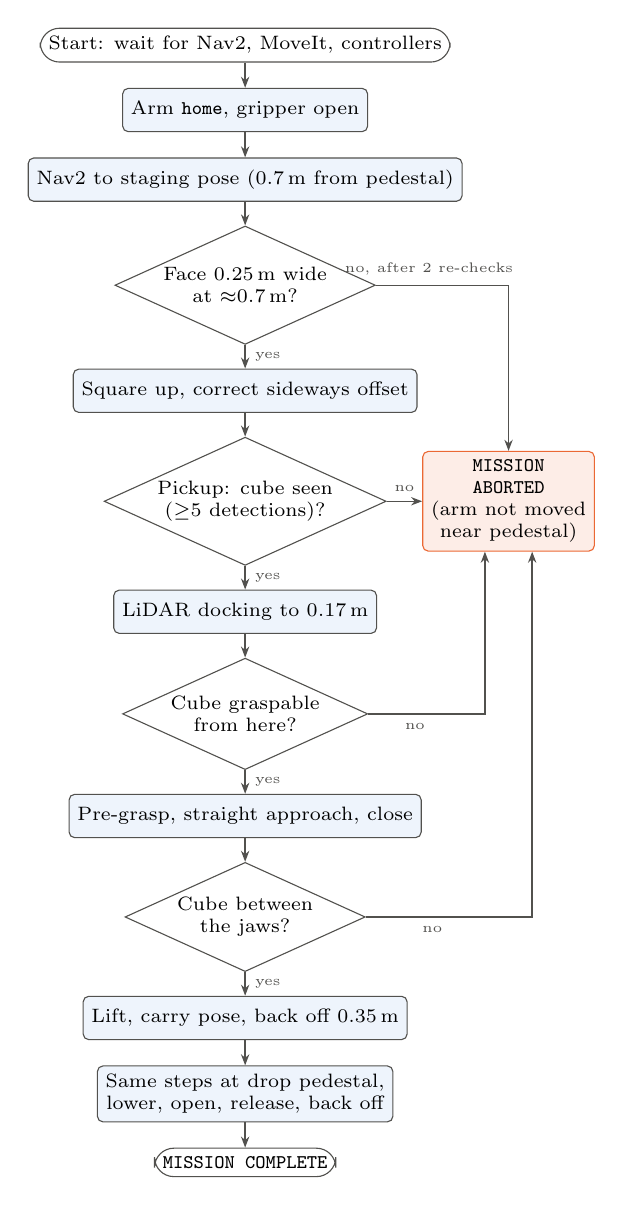
\begin{tikzpicture}[node distance=0.32cm]
  \node[term] (s) {Start: wait for Nav2, MoveIt, controllers};
  \node[box, below=of s] (home) {Arm \texttt{home}, gripper open};
  \node[box, below=of home] (nav) {Nav2 to staging pose (\SI{0.7}{m} from pedestal)};
  \node[decision, below=0.3cm of nav] (loc) {Face \SI{0.25}{m} wide\\ at $\approx$\SI{0.7}{m}?};
  \node[box, below=0.3cm of loc] (lat) {Square up, correct sideways offset};
  \node[decision, below=0.3cm of lat] (cam) {Pickup: cube seen\\ ($\geq$5 detections)?};
  \node[box, below=0.3cm of cam] (dock) {LiDAR docking to \SI{0.17}{m}};
  \node[decision, below=0.3cm of dock] (reach) {Cube graspable\\ from here?};
  \node[box, below=0.3cm of reach] (grasp) {Pre-grasp, straight approach, close};
  \node[decision, below=0.3cm of grasp] (att) {Cube between\\ the jaws?};
  \node[box, below=0.3cm of att] (lift) {Lift, carry pose, back off \SI{0.35}{m}};
  \node[box, below=of lift] (drop) {Same steps at drop pedestal,\\ lower, open, release, back off};
  \node[term, below=of drop] (done) {\texttt{MISSION COMPLETE}};

  \node[stop, right=0.45cm of cam] (abort) {\texttt{MISSION}\\ \texttt{ABORTED}\\ (arm not moved\\ near pedestal)};

  \foreach \a/\b in {s/home, home/nav, nav/loc, lat/cam, dock/reach, grasp/att, lift/drop, drop/done}
    \draw[arr] (\a) -- (\b);
  \draw[arr] (loc) -- node[lbl, right]{yes} (lat);
  \draw[arr] (cam) -- node[lbl, right]{yes} (dock);
  \draw[arr] (reach) -- node[lbl, right]{yes} (grasp);
  \draw[arr] (att) -- node[lbl, right]{yes} (lift);
  \draw[arr] (loc.east) -| node[lbl, above, pos=0.2]{no, after 2 re-checks} (abort.north);
  \draw[arr] (cam.east) -- node[lbl, above]{no} (abort.west);
  \draw[arr] (reach.east) -| node[lbl, below, pos=0.2]{no} ([xshift=-0.3cm]abort.south);
  \draw[arr] (att.east) -| node[lbl, below, pos=0.2]{no} ([xshift=0.3cm]abort.south);
\end{tikzpicture}
\caption{Mission flowchart with the run-time safety checks. The drop pedestal repeats the drive, check and docking steps without the camera step.}
\label{fig:flow}
\end{figure}

\subsection{Two-stage parking}
\label{sec:parking}
The arm grasps about \SI{20}{cm} in front of the base, and the graspability check (\cref{sec:checks}) accepts the cube only within a \SI{3.5}{cm} deep window. The robot therefore has to stop within about \SI{1}{cm} and \SI{2}{\degree} of the right place. Nav2 cannot do this reliably. Its goal tolerance is \SI{10}{cm}, a differential-drive robot cannot move sideways, and with the earlier DWB controller the robot often stopped \SIrange{0.15}{0.3}{m} short when the goal was close to an obstacle. Parking is therefore split into two stages (\cref{fig:dock}).

\begin{figure}[t]
\centering
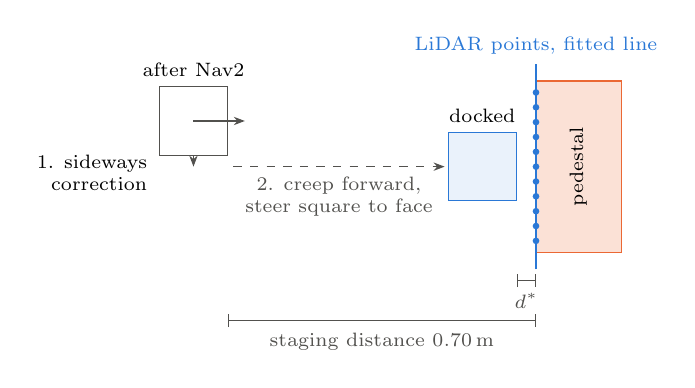
\begin{tikzpicture}[x=1.45cm, y=1.45cm, font=\scriptsize]
  \fill[corange!20, draw=corange] (3.6,-0.75) rectangle (4.35,0.75);
  \node[rotate=90] at (3.97,0) {pedestal};
  \foreach \y in {-0.65,-0.52,...,0.66} \fill[cblue] (3.6,\y) circle (1.2pt);
  \draw[cblue, line width=0.8pt] (3.6,-0.9) -- (3.6,0.9);
  \node[cblue, anchor=south] at (3.6,0.9) {LiDAR points, fitted line};
  \draw[cgray, fill=white] (0.3,0.1) rectangle (0.9,0.7);
  \draw[arr] (0.6,0.4) -- (1.05,0.4);
  \node[anchor=south] at (0.6,0.7) {after Nav2};
  \draw[cblue, fill=cblue!10] (2.83,-0.3) rectangle (3.43,0.3);
  \node[anchor=south] at (3.13,0.3) {docked};
  \draw[arr, dashed] (0.6,0.1) -- (0.6,-0.0);
  \node[anchor=east, align=right] at (0.28,-0.05) {1. sideways\\ correction};
  \draw[arr, dashed] (0.95,0) -- (2.8,0) node[midway, below, align=center]{2. creep forward,\\ steer square to face};
  \draw[|-|, cgray] (3.43,-1.0) -- (3.6,-1.0) node[midway, below=1pt]{$d^\ast$};
  \draw[|-|, cgray] (0.9,-1.35) -- (3.6,-1.35) node[midway, below=1pt]{staging distance \SI{0.70}{m}};
\end{tikzpicture}
\caption{Two-stage parking. Nav2 stops at a staging pose. The docking step fits a line to the LiDAR points on the pedestal face, removes the sideways offset (turn \SI{90}{\degree}, drive, turn back), and creeps forward while steering perpendicular to the face.}
\label{fig:dock}
\end{figure}

\paragraph*{Stage 1, Nav2} Nav2 drives to a staging pose \SI{0.70}{m} in front of the pedestal, in open space where it reliably arrives.

\paragraph*{Stage 2, LiDAR docking} The LiDAR points within \SI{60}{\degree} of straight ahead are converted to the base frame. Only the nearest \SI{7}{cm} deep band is kept, which is the pedestal's front face. A least-squares line $x = a + b\,y$ is fitted to these points. From it follow the heading error $\psi = -\arctan b$, the perpendicular distance $d = a\cos(\arctan b)$, the face width, and the sideways offset (the centre of the face's $y$ extent). If the offset exceeds \SI{1.5}{cm}, the robot turns \SI{90}{\degree}, drives the offset and turns back, up to three times. It then creeps forward with
\begin{align}
  \omega &= \mathrm{sat}_{\pm 0.4}(1.5\,\psi),\\
  v &= \begin{cases} 0, & |\psi| > 8^\circ,\\
  \mathrm{sat}_{[-0.05,\,0.08]}\bigl(0.6\,(d - d^\ast)\bigr), & \text{otherwise},\end{cases}
\end{align}
with $d^\ast = \SI{0.17}{m}$, and stops after three consecutive scans with $|d-d^\ast| < \SI{1}{cm}$ and $|\psi| < \SI{2}{\degree}$.

\subsection{Cube detection}
\label{sec:camera}
When the robot is docked, the cube is above the camera's field of view. The camera therefore looks for it at the staging pose, \SI{0.7}{m} away, and the mission stores the result in the odometry frame. Odometry drift over the remaining \SI{0.5}{m} is negligible. For each synchronized colour and depth frame (\cref{fig:cam}):
\begin{enumerate}
  \item threshold saturated red in HSV (two hue bands, $S \geq 120$, $V \geq 60$) and apply a $3{\times}3$ morphological opening;
  \item take the largest blob above \SI{40}{px} as the cube's visible front face;
  \item take the median depth $z$ over the blob;
  \item back-project the blob centroid $(u,v)$ with the pinhole model~\cite{hartley2004mvg}, $x = (u-c_x)z/f_x$, $y = (v-c_y)z/f_y$, and move half a cube further along the horizontal viewing ray to reach the centre;
  \item transform the point to the odometry frame and publish it.
\end{enumerate}
The mission takes the median of at least five detections collected while the robot stands still.

\begin{figure}[t]
\centering
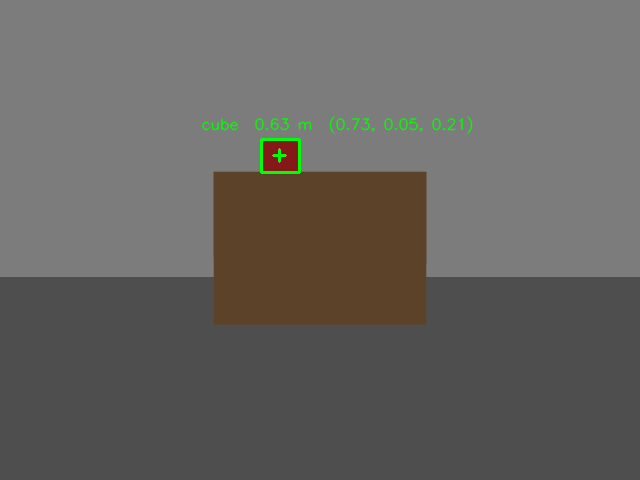
\includegraphics[width=0.78\columnwidth]{cube_detection.png}\\[3pt]
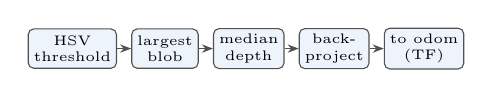
\begin{tikzpicture}[node distance=0.18cm, every node/.style={box, font=\tiny, minimum height=0.5cm, inner sep=2pt}]
  \node (a) {HSV\\ threshold};
  \node[right=of a] (b) {largest\\ blob};
  \node[right=of b] (c) {median\\ depth};
  \node[right=of c] (d) {back-\\ project};
  \node[right=of d] (e) {to odom\\ (TF)};
  \foreach \p/\q in {a/b,b/c,c/d,d/e} \draw[arr] (\p) -- (\q);
\end{tikzpicture}
\caption{Cube detection. Top: the camera view from the staging pose, with the detected cube (here \SI{5}{cm} off-centre), its distance and 3D position. Bottom: processing steps.}
\label{fig:cam}
\end{figure}

\subsection{Arm kinematics and motion}
The OpenMANIPULATOR-X has a base yaw joint $q_1$ followed by three pitch joints $q_2, q_3, q_4$ in one vertical plane. For a target point $(x,y,z)$ of the end effector in the base frame and a desired gripper pitch $\phi$, the solution is closed form~\cite{spong2006robot}. With joint~1 at $x_1 = \SI{-0.080}{m}$ and the shoulder at height $h = \SI{0.1775}{m}$:
\begin{align}
  q_1 &= \operatorname{atan2}(y,\; x - x_1), \qquad r = \sqrt{(x-x_1)^2 + y^2},\\
  w_x &= r - \ell_e\cos\phi, \qquad w_z = z - h - \ell_e\sin\phi,\\
  \cos\delta &= \frac{w_x^2 + w_z^2 - a^2 - b^2}{2ab},\\
  t_1 &= \operatorname{atan2}(w_z, w_x) + \operatorname{atan2}(b\sin\delta,\; a + b\cos\delta),\\
  t_2 &= t_1 - \delta,\\
  q_2 &= \alpha - t_1,\qquad q_3 = -t_2 - q_2,\qquad q_4 = t_2 - \phi,
\end{align}
where $a = \SI{0.130}{m}$ is the length of the first (offset) link, $\alpha = \operatorname{atan2}(0.128, 0.024)$ its angle, $b = \SI{0.124}{m}$ the second link and $\ell_e = \SI{0.126}{m}$ the wrist-to-tool length. The elbow-up branch is used, and solutions outside the joint limits are rejected.

In testing, MoveIt's sampling-based planner occasionally produced large detours, and once swung the open gripper into the cube, because its planning scene did not contain the cube or the pedestals. Near the pedestals, all arm motions are therefore deterministic:
\begin{itemize}
  \item \textbf{Straight lines} for approach, lift, lower and retreat: inverse kinematics at ten waypoints, sent as one joint trajectory.
  \item \textbf{Evenly interpolated joint moves} to and from the pre-grasp pose, with the fingertip path checked in advance to stay \SI{2}{cm} clear of the cube.
\end{itemize}
The grasp stops \SI{8}{mm} short of the cube centre and \SI{5}{mm} above it, which keeps the wide gripper palm in front of the pedestal edge.

\subsection{Gripper and grasp assist}
\label{sec:grasp}
The finger links in the ROBOTIS model weigh only \SI{1}{g}. With position-controlled fingers, Gazebo moved the fingers straight into the cube and ODE pushed it off the pedestal. In one test a finger was reported at \SI{0.077}{m} on a joint limited to \SI{0.019}{m}. Both fingers are therefore effort-controlled by one \texttt{JointGroupEffortController} (open $+\SI{0.4}{N}$, close $-\SI{0.2}{N}$). The right finger is no longer a mimic joint, because in Humble's \texttt{gazebo\_ros2\_control} a mimic joint only copies position commands.

Squeezing a light cube between effort-controlled \SI{1}{g} fingers was still not stable in ODE. A small Gazebo plugin therefore provides \texttt{attach} and \texttt{detach} services. On \texttt{attach} it first checks that the cube lies between the jaws (within $\pm$\SI{3}{cm}, $\pm$\SI{1.5}{cm} and $\pm$\SI{2}{cm} of the grasp point in the gripper frame), and only then fixes it to the gripper with a joint. The robot still has to park, aim the arm and close the fingers correctly; only the holding friction is replaced. A real gripper would not need this step, and it is the main limitation of the grasping results.

\subsection{Run-time safety checks}
\label{sec:checks}
\begin{itemize}
  \item \textbf{Localization check} on arrival at each staging pose: the LiDAR must see a face about \SI{0.25}{m} wide ($\pm$\SI{9}{cm}) at about \SI{0.7}{m} ($\pm$\SI{25}{cm}). The robot first waits until odometry shows it is still, and re-measures twice before failing.
  \item \textbf{Graspability check:} the cube's front face must lie between \SI{1}{cm} in front of and \SI{2.5}{cm} behind the pedestal edge, and at most \SI{11}{cm} to the side.
  \item \textbf{Path check} for joint moves near the cube (above).
  \item \textbf{Grasp check:} the attach service refuses if the cube is not between the jaws.
\end{itemize}

% =====================================================================
\section{Implementation}
\label{sec:problems}

The project consists of five ROS~2 packages (description, bring-up, navigation, MoveIt configuration, perception) plus the unmodified ROBOTIS package. The mission node uses simulation time throughout, so its time-outs stay valid when the simulation runs slower than real time. A GitHub Actions workflow builds the workspace in a clean \texttt{ros:humble} container on every push. Scripts reproduce the evaluation (\texttt{tools/run\_trials.sh}) and the demo video (\texttt{tools/record\_demo.sh}).

Most of the engineering effort went into problems that appeared only in repeated testing. \Cref{tab:problems} lists them. Each one caused at least one failed run before it was fixed.

\begin{table}[t]
\caption{Problems Found by Repeated Testing}
\label{tab:problems}
\centering
\footnotesize
\begin{tabular}{@{}L{0.49\columnwidth}L{0.46\columnwidth}@{}}
\toprule
Problem & Fix \\
\midrule
DWB controller stopped \SIrange{0.15}{0.3}{m} short of goals & Regulated Pure Pursuit + two-stage parking \\
Position-controlled fingers teleported into the cube & effort-controlled fingers \\
Mimic finger went limp under effort control & both fingers in one effort controller \\
ODE unstable with \SI{1}{g} finger links & grasp assist plugin \\
Detaching while squeezing threw the cube & open first, then detach \\
Gripper palm clipped the pedestal edge & stop \SI{8}{mm} short, \SI{5}{mm} high \\
MoveIt detours, gripper swung into cube & straight-line and checked joint moves \\
Real-time time-outs cut moves short & mission uses simulation time \\
Nav2/AMCL never activated (Fast DDS) & Cyclone DDS \\
Localization check fooled by a scan taken while moving & wait until still, re-check \\
Detector could not transform images (TF thread blocked) & TF listener in its own thread \\
TF listener thread crashed \texttt{rclpy} & TF listener on its own node \\
\texttt{bt\_navigator} failed to start under load & action-server wait \SI{1}{s} $\to$ \SI{5}{s} \\
\bottomrule
\end{tabular}
\end{table}

% =====================================================================
\section{Experiments and Results}

\subsection{Method}
Every run is a full mission in a freshly started, headless simulation on an 8-core laptop, where the simulation ran at about 0.3--0.5$\times$ real time. The \textbf{success criterion is ground truth from Gazebo}: after the run, the cube must stand upright on the drop pedestal. The mission's own \texttt{MISSION COMPLETE} message is not used, and \cref{sec:undetected} shows why. Parking and grasp values come from the mission's logs. Camera errors are measured against the cube position set in Gazebo before the run.

The data come from 22 runs in five groups, made during development (\cref{tab:runs}). They are not one controlled experiment: the software changed between groups, and the groups had different purposes. For the camera runs the cube was placed at random on the pickup pedestal, up to $\pm$\SI{5}{cm} sideways and $\pm$\SI{15}{\degree} turned; in the other groups it was at its default place. Logs for the five earliest runs (P1--P5) were not kept, so they contribute only their outcomes. The extraction script and the data are in the repository~\cite{repo}.

\begin{table}[t]
\caption{Evaluation Runs}
\label{tab:runs}
\centering
\footnotesize
\setlength{\tabcolsep}{4pt}\begin{tabular}{@{}llcL{0.27\columnwidth}@{}}
\toprule
Runs & Software state & Cube & Purpose \\
\midrule
P1--P5 & before camera & fixed & repeatability \\
T1--T5 & before camera & fixed & localization tracking \\
F1 & before camera & fixed & fresh clone \\
C1--C8 & camera, in development & random & camera validation \\
C9--C11 & final software & random & demo, script and fresh-clone checks \\
\bottomrule
\end{tabular}
\end{table}

\subsection{Overall outcome}
\begin{figure}[t]
\centering
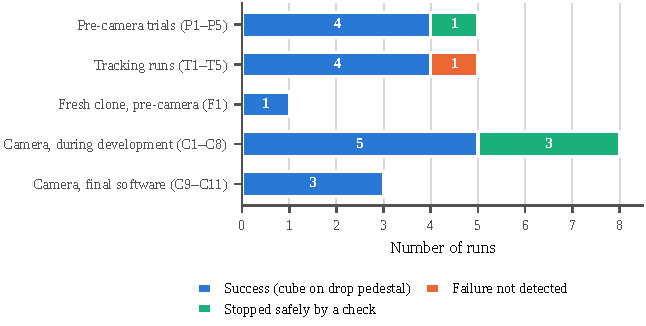
\includegraphics[width=\columnwidth]{outcomes.pdf}
\caption{Outcome of all 22 runs, judged by the cube's final position in Gazebo.}
\label{fig:outcomes}
\end{figure}

\Cref{fig:outcomes} summarizes the outcomes: 17 of 22 runs succeeded, and 13 of the 17 runs with logs. Four runs were stopped safely by a check before the arm moved near the pedestal, and the cause of each was fixed:
\begin{itemize}
  \item \textbf{P3:} AMCL localized the robot wrongly at start-up, and the grasp check found no cube between the jaws. This led to the localization check.
  \item \textbf{C1:} a detector left running from an earlier test published positions in the wrong frame, which the graspability check rejected. The mission now accepts only odometry-frame detections.
  \item \textbf{C2:} the localization check saw a face only \SI{14}{cm} wide, most likely from a scan taken while the robot was still slowing down. The check now waits for standstill and re-measures.
  \item \textbf{C6:} the camera produced no usable detections because the detector's TF listener was blocked, and the mission stopped with ``cube not found''.
\end{itemize}
One run (T5) failed without the robot noticing; it is discussed in \cref{sec:undetected}. All three runs with the final software (C9--C11) succeeded. A fourth successful run with the final software was watched in the Gazebo window, but its full log was not saved, so it is not counted.

\subsection{Parking accuracy}
\begin{figure}[t]
\centering
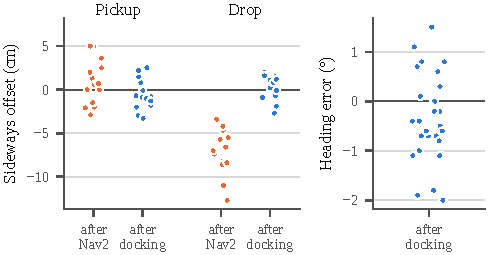
\includegraphics[width=\columnwidth]{parking.pdf}
\caption{Parking accuracy over all logged runs. Left: sideways offset to the pedestal centre after Nav2 (orange) and after LiDAR docking (blue). Right: heading error after docking.}
\label{fig:parking}
\end{figure}

\Cref{fig:parking} and \cref{tab:parking} show the effect of the docking stage. Nav2 alone arrived at the pickup staging pose with a mean absolute sideways offset of \SI{2.0}{cm} (maximum \SI{5.0}{cm}). At the drop pedestal it was consistently off to one side, by \SI{7.2}{cm} on average and up to \SI{12.7}{cm}, which is more than the arm can reach. After docking, the mean absolute sideways offset was \SIrange{1.2}{1.6}{cm} (maximum \SI{3.3}{cm}), the heading error was at most \SI{2.0}{\degree}, and the distance to the face was \SIrange{0.167}{0.180}{m}. The distance is systematically about \SI{8}{mm} above the \SI{0.17}{m} target because docking stops as soon as it is within its \SI{1}{cm} tolerance. The remaining sideways offset is handled by joint~1, which turns the arm towards the cube.

\begin{table}[t]
\caption{Parking Accuracy (Mean Absolute Value / Maximum; Pickup $n{=}16$ After Nav2, 15 After Docking; Drop $n{=}14$)}
\label{tab:parking}
\centering
\footnotesize
\setlength{\tabcolsep}{3pt}\begin{tabular}{@{}lcccc@{}}
\toprule
& \multicolumn{2}{c}{Sideways offset (cm)} & Heading & Distance \\
\cmidrule(lr){2-3}
Pedestal & after Nav2 & after docking & error (°) & (m) \\
\midrule
Pickup & 2.0 / 5.0 & 1.6 / 3.3 & 0.7 / 1.8 & 0.167--0.180 \\
Drop & 7.2 / 12.7 & 1.2 / 2.7 & 0.9 / 2.0 & 0.174--0.180 \\
\bottomrule
\end{tabular}
\end{table}

\subsection{Cube localization and grasp}
\begin{figure}[t]
\centering
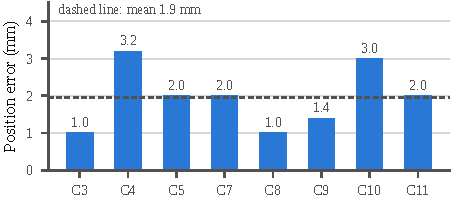
\includegraphics[width=\columnwidth]{camera_error.pdf}
\caption{Horizontal error of the camera's cube position against the position set in Gazebo, for every camera run that reached the grasp (C1 excluded, see text).}
\label{fig:camera}
\end{figure}

\Cref{fig:camera} shows the camera's position error for the eight camera runs that reached the grasp. The error was \SIrange{1.0}{3.2}{mm}, with a mean of \SI{1.9}{mm}, for cubes placed up to \SI{4.4}{cm} off-centre and turned up to \SI{14}{\degree}. Run C1 is excluded because its detections came from the leftover test process, not from the evaluated detector. Of 19 localization checks in the logs, 18 passed: the face was measured at \SIrange{0.23}{0.25}{m} wide and \SIrange{0.71}{0.77}{m} away. The one failure was C2.

In all 14 logged grasps, the grasp assist confirmed the cube between the jaws. The cube's offset from the grasp point was at most \SI{1.1}{cm}, and it was mainly the intended \SI{8}{mm} stop-short.

\subsection{Mission time}
\begin{figure}[t]
\centering
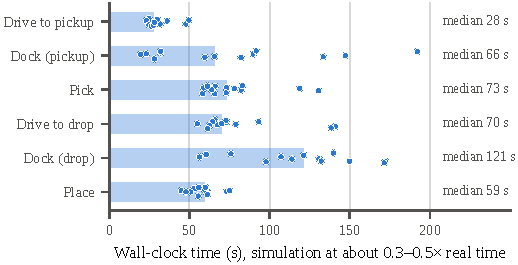
\includegraphics[width=\columnwidth]{phases.pdf}
\caption{Duration of each mission phase in the 13 successful logged runs (dots), with the median (bar).}
\label{fig:phases}
\end{figure}

A complete mission took a median of \SI{414}{s} of wall-clock time (\SIrange{275}{736}{s}), at 0.3--0.5$\times$ real time. As \cref{fig:phases} shows, docking at the drop pedestal was the longest and most variable phase (median \SI{121}{s}). It is the phase that had to remove Nav2's large sideways offset, often in two or three correction steps.

\subsection{Undetected failure}
\label{sec:undetected}
In run T5, the physics became unstable at the drop pedestal while the cube was being released. The arm reached the place pose, the gripper opened with the cube still attached by the grasp assist, and the cube was detached \SI{7.4}{s} later. Between two ground-truth samples that bracket the moment of release, the robot was thrown more than \SI{10}{m}, out of the arena, and the cube ended on the floor far outside it. Whether the instability started while the fingers opened or at the detach itself cannot be told from the samples. The mission did not notice. Its remaining steps raised no error, so it reported \texttt{MISSION COMPLETE}. This is the most important negative result: the release step has no check, and an internal success message is not evidence of success. Possible fixes are discussed in \cref{sec:future}.

\subsection{Reproducibility}
The repository was cloned from GitHub into an empty folder and set up by following only its README, with no settings from the development machine. All 13 packages built, and a full mission with a randomly placed cube succeeded (C11). Checking the README against the packages' declared dependencies showed that three dependencies of the ROBOTIS package were missing from its installation list. The README now installs them with \texttt{rosdep}, the same step the CI runs in a clean container.

% =====================================================================
\section{Discussion}

\paragraph*{What worked} Splitting parking into a coarse Nav2 stage and a fine docking stage was the key design decision. It turns a \SIrange{3}{13}{cm} navigation error into about \SI{1}{cm}, which a short arm can handle. Looking for the cube from the staging pose, where it is fully visible, gives millimetre accuracy with a very simple colour detector. Making all arm motions near the pedestals deterministic removed a whole class of random failures. The safety checks did their job: in four runs they stopped the mission before the arm could hit anything, and each stop pointed directly to a fixable cause.

\paragraph*{Threats to validity} The evidence is limited in several ways that the reader should weigh:
\begin{itemize}
  \item \textbf{Small, heterogeneous sample.} 22 runs in five groups, with the software changing between groups. Only three logged runs used the final software, so the success rate of the final system is not well established.
  \item \textbf{Grasp assist.} Holding the cube is simulated by a fixed joint. The grasp results show that the robot reaches the right place with the gripper closed around the cube; they say nothing about grip stability on real hardware.
  \item \textbf{Contaminated runs.} Test processes left over from earlier runs, such as old detectors and an obsolete initial-pose publisher, were found running during the camera runs C1--C8. C1 was visibly affected and is excluded from the accuracy figures. The others ran on the same camera images and are believed unaffected, but they were not fully clean. The cleanup has since been fixed.
  \item \textbf{Simple world.} One known object of a distinctive colour, static obstacles, and ideal lighting.
\end{itemize}

\paragraph*{Comparison with the objectives} Objectives 1 to 3 are met in simulation. Objective~4 is met for the pick side but not for the release, as T5 shows. Objective~5 is met: the outcomes are judged by ground truth, failures are reported, and a fresh clone builds and runs.

% =====================================================================
\section{Conclusion and Future Work}
\label{sec:future}
A complete autonomous pick-and-place mission was built and evaluated in simulation from standard ROS~2 components and a small number of purpose-built parts: two-stage LiDAR docking, a colour-and-depth cube detector, analytic inverse kinematics with straight-line motions, and run-time safety checks. Thirteen of 17 logged runs succeeded. Docking reduced the parking error to about \SI{1}{cm}, and the camera located the cube within \SI{3.2}{mm}.

Future work, in order of priority:
\begin{enumerate}
  \item \textbf{Check the release:} verify after placing that the cube is on the pedestal (with the camera from the staging pose) and that odometry shows no jump. Investigate the instability, for example by detaching before the fingers move.
  \item \textbf{A clean, larger evaluation} with the final software, using the included trial script.
  \item \textbf{Recovery instead of abort:} back off and retry after a failed check, for example with a behaviour tree.
  \item \textbf{Real grasp physics} without the attachment plugin, for example in the newer Gazebo or with tuned contact parameters, and then real hardware.
  \item \textbf{More general perception:} several and unknown objects, learned detection, and grasp pose estimation.
\end{enumerate}

% =====================================================================
\appendices
\section{Main Parameters}
\begin{table}[h]
\centering
\footnotesize
\setlength{\tabcolsep}{4pt}\begin{tabular}{@{}lL{0.52\columnwidth}@{}}
\toprule
Parameter & Value \\
\midrule
Nav2 controller & Rotation Shim + RPP, \SI{10}{Hz}, \SI{0.20}{m/s} \\
Nav2 goal tolerance & \SI{0.10}{m}, \SI{0.10}{rad} \\
AMCL & likelihood field, 500--2000 particles \\
Costmap resolution / inflation & \SI{0.05}{m} / \SI{0.55}{m} \\
Staging / docking / back-off & \SI{0.70}{m} / \SI{0.17}{m} / \SI{0.35}{m} \\
Docking stop tolerance & \SI{1}{cm}, \SI{2}{\degree}, 3 scans \\
Camera & 640\,$\times$\,480\,px, \SI{62}{\degree}, \SI{10}{Hz}, $\sigma_z$ = \SI{5}{mm} \\
Detector & $S \geq 120$, $V \geq 60$, blob $\geq$ \SI{40}{px}, median of $\geq 5$ \\
Gripper effort & open $+\SI{0.4}{N}$, close $-\SI{0.2}{N}$ \\
Grasp offset & \SI{8}{mm} short, \SI{5}{mm} high; pre-grasp \SI{7}{cm} \\
Middleware & Cyclone DDS \\
\bottomrule
\end{tabular}
\end{table}

\section{Reproducing the Results}
On Ubuntu~22.04 with ROS~2 Humble, follow the README of~\cite{repo}: clone the repository and the ROBOTIS package at commit \texttt{814f140}, install the dependencies with \texttt{apt} and \texttt{rosdep}, and build with \texttt{colcon}. Then \texttt{tools/run\_trials.sh N} runs $N$ missions with a randomly placed cube and judges each by Gazebo ground truth. The figures in this report are generated by \texttt{docs/report/data/extract\_runs.py} and \texttt{docs/report/figures/make\_figures.py}.

\bibliographystyle{IEEEtran}
\bibliography{refs}

\end{document}
